\documentclass[12pt]{article}
\usepackage{graphicx}
\usepackage{caption}
\usepackage{subcaption}
\usepackage{tikz}
\usepackage{venndiagram}
\usepackage{venndiagram}
\usepackage{tcolorbox}
\usepackage{listings}
\usepackage{enumitem}
\usepackage{amsmath}
\usepackage{amssymb}
\usepackage{colortbl}
\usepackage{xcolor}
\usepackage[margin=1cm, top=1.5cm, bottom=1.5cm]{geometry}

\tcbuselibrary{breakable}

\title{\textbf{Gráficas y Juegos: Tarea 06}}
\author{Martínez Méndez Ángel Antonio\\Pinzón Chan José Carlos\\Rendón Ávila Jesús Mateo}
\date{\today}

\begin{document}

\maketitle
\begin{center}
\vspace{3cm}
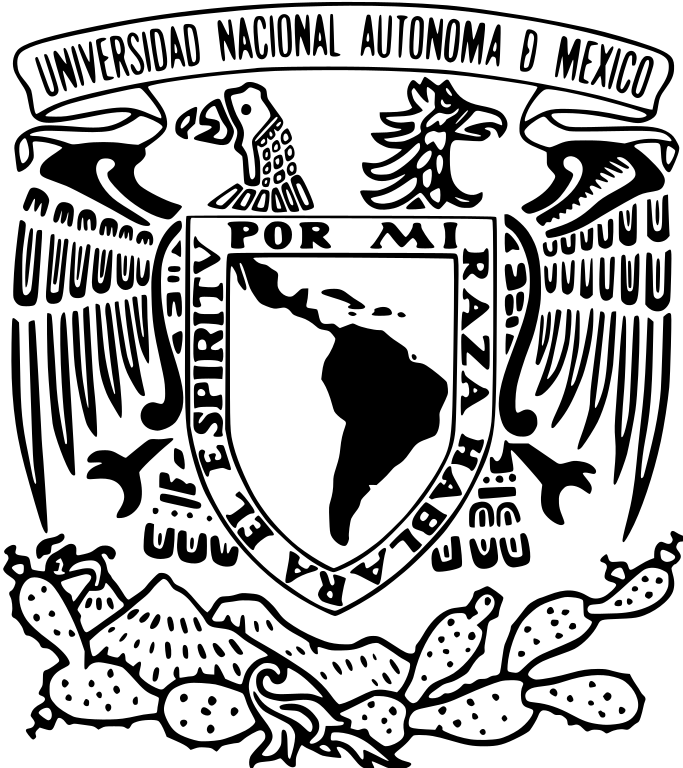
\includegraphics[width=0.195\textwidth]{Escudo.png}
\hspace{0.5cm}
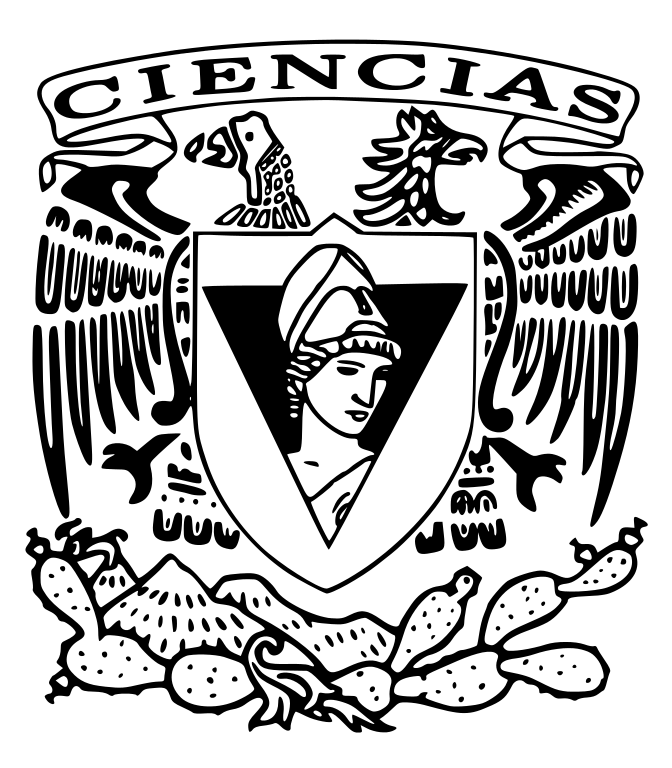
\includegraphics[width=0.2\textwidth]{logo_ciencias.png}
\end{center}
\begin{center}
    \vspace{1cm}
    Universidad Nacional Autónoma de México\\
    Facultad de Ciencias\\
    Profesor: César Hernández Cruz\\
\end{center}

\newpage

%
% Ejercicio 1
%
\textbf{1.} Sea $G$ una gráfica conexa no euleriana. Demuestre que las siguientes afirmaciones son equivalentes.
\begin{enumerate}

\item[$1)$] Hay un paseo euleriano en $G$.

\item[$2)$] Hay exactamente dos vértices de grado impar en $G$.

\item [$3)$]Existe una familia de ciclos ajenos por aristas dos a dos $\{C_i \}_{i=1}^k$ y un paseo $P$, ajeno por aristas a cada uno de los ciclos en la familia anterior, tales que $E_G = E_P \cup \bigcup_{i=1}^k E_{C_i}$.

\end{enumerate}
\begin{tcolorbox}[title=\textbf{Hipótesis (General)}, colback=red!15!white, colframe=black!]
	
$G$ es una gráfica conexa y no euleriana.
 
\end{tcolorbox}
	
\begin{tcolorbox}[title=\textbf{Definiciones}, colback=blue!15!white, colframe=black!]
     $Def$. Un paseo euleriano $T$ de una gráfica $G$, es un paseo tal que $E_T = E_G$ 
\end{tcolorbox}



\textbf{Demostracion $1) \Rightarrow 2)$}\\

Podemos suponer que $G$ no es trivial.\\

Dado que $G$ no es euleriana, al menos el grado de algún vértice de $G$ es impar. Como $G$ tiene un paseo euleriano $P$, sea $P$ = $(x_0,x_1,...,x_n)$, donde $x_0 \neq x_n$, entonces $P$ no repite aristas. Si agregamos un vértice $v$ tal que sea adyacente a $x_0$ y a $x_n$ podemos dar el siguiente circuito euleriano: $C = x_0Px_nvx_0$. Sabemos que el circuito es euleriano porque $P$ utiliza todas las aristas de $G$, no repite ninguna y además las aristas $x_0v$ y $x_nv$ no existén en $G$, por lo que no han sido utilizadas previamente. Como esta nueva gráfica  \{$G + v$\} es euleriana, eso significa que los grados de todos los vértices son pares, es decir, los vértices impares aumentaron su grado y se volovieron pares. Los únicos vértices de $G$ que aumentaron sus grados fueron $x_0$ y $x_n$, más especificamente en una unidad. Al sumar impar más impar se obtiene un número par, por consiguiente, tiene que ser que $x_0$ y $x_n$ tengan grados impares, pues en otro caso se contradice que \{$G + v$\} sea euleriana (Si $x_0$ o $x_n$ fueran pares, al agregar a $v$ y sus aristas, la gráfica tendría un circuito euleriano, pero los vértices se volverían impares, lo cual no tiene sentido).\\

$\therefore$ Hay exactamente dos vértices de grado impar en $G$.\\

\textbf{Demostracion $2) \Rightarrow 3)$}\\

Como hay exactamente dos vértices de grado impar en $G$ , dígase $x$ y $y$, y $G$ es conexa, entonces podemos afirmar que existe una xy-trayectoria $T$ en $G$ (observe que esta trayectoria es también un paseo). Si obtenemos la subgráfica $G - E_T$, los vértices con grado par en $T$ pierden exactamente dos aristas, por lo que su grado sigue siendo par (o cero). En el caso de los vértices extremos  estos pierden una arista, de modo que su grado ahora es par (o cero). Como por hipótesis $G$ sólo tiene dos vértices de grado impar ($x$,$y$) y en la subgráfica $G - E_T$ para todo $u \in V_T$ se cumple que el grado de $u$ es par, entonces para todo $v \in V_{G - E_T}$ el grado de $v$ es par.\\

Ahora bien, como todo vértice en $G - E_T$ es par, entonces $G - E_T$ admite una descomposición en ciclos ajenos  por aristas dos a dos $\{C_i \}_{i=1}^k$; además son ajenos por aristas a la trayectoria $T$. Finalmente si unimos las arista de los ciclos y de la trayectoria $T$:  $E_T \cup \bigcup_{i=1}^k E_{C_i}$ = $E_T \cup E_{G-T} $ = $E_G$.\\

$\therefore$ Existe una familia de ciclos ajenos por aristas dos a dos $\{C_i \}_{i=1}^k$ y un paseo $P$, ajeno por aristas a cada uno de los ciclos en la familia anterior, tales que $E_G = E_P \cup \bigcup_{i=1}^k E_{C_i}$.\\

\textbf{Demostracion $3) \Rightarrow 1)$}\\
Dado que la gráfica tiene una descomposición en ciclos y un paseo $P = (x_0,...,x_n)$, decimos que $G - E_P$, es una subgráfica con una descomposición en ciclos y todos los vértices con grado par (como se mostró en $2) \Rightarrow 3)$). Por lo tanto $G - E_P$ es una subgráfica euleriana de $G$.\\

Como $G - E_P$ tiene un circuito euleriano $C$ que empieza en un vértice arbitrario, sea este vértice un vértice extremo de $P$ (ya sea $x_0$ o $x_n$), entonces podemos recorrer todas las aristas de $G - E_P$ partiendo de (por ejemplo) $x_0$ y regresando a dicho  vértice; esto es: $C = (x_0,...,x_k,x_0)$ donde evidentemente ninguna arista de $C$ es arista de $P$.\\

Finalmente, al regresar a nuestra gráfica $G$, el paseo euleriano $Q$ de $G$ se describe como: $Q = x_0Cx_0Px_n$. Quiero destacar algunos puntos importantes:

\begin{enumerate}

\item[$1)$] El circuito euleriano $C$ "recorre" todas las aristas de  $G - E_P$, por lo tanto al recorrer este circuito y después el paseo $P$, ya hemos utilizado todas las aristas de $G$ una única vez.

\item[$2)$]Si el grado de que $x_0$ es 1, entonces el circuito $C$ comienza en el vértice adyacente a $x_0$, sea este vértice $x_1$ entonces $C = (x_1,...,x_k,x_1)$. En este caso el paseo euleriano $Q$ queda descritó como: $Q = x_0x_1Cx_1Px_n$.

\item[$3)$] Todo lo anterior es análogo para $x_n$.

$\therefore$  Hay un paseo euleriano en $G$.

\end{enumerate}

\vspace{1cm}

%
% Ejercicio 2
%
\textbf{2}. Sea $D$ una digráfica conexa. Demuestre que D es euleriana si y solo si para cada 
vértice $v \in D$ se tiene que $d^+(v) = d^-(v)$.

\begin{tcolorbox}[title=\textbf{Hipotesis}, colback=red!15!white, colframe=black!]
    $D$ es una digráfica conexa.
\end{tcolorbox}

\begin{tcolorbox}[title=\textbf{Definiciones}, colback=blue!15!white, colframe=black!]
    $Def.$ Una digráfica es \textbf{euleriana} si tiene un circuito euleriano.\\

    $Def.$ Un \textbf{circuito euleriano} es un paseo euleriano cerrado que utiliza todas las flechas 
    de $D$.

\end{tcolorbox}

\textbf{Demostración.}

\textcolor{blue}{$[\Rightarrow]$} Sea $D$ una digráfica euleriana. Al tener un circuito cerrado quiere 
decir que la digráfica utiliza todas las flechas de $D$; iniciando en un vértice arbitrario $v \in D$ 
y terminando en el mismo.\\

Dado que la digráfica es euleriana, toda flecha que entre en un vértice arbitrario $v \in V_D$, tal que 
$u \rightarrow v \in A_D$, tiene que salir de salir de esta misma $v \rightarrow w \in A_D$. En dado caso de 
que inciemos en un vértice $x$, por hipótesis, al ser conexa $D$, en algún momento existirá una flecha 
que regrese al vértice $x$.\\

Por lo que para todo vértice arbitrario $v \in V_D$ se tiene que $d^+(v) = d^-(v)$. Esta última 
afirmación nos da la propiedad análoga en las gráficas eulerianas, en las cuales todos sus vértices tienen 
grádo par.\\

\textcolor{blue}{$[\Leftarrow]$} Sea $D$ una digráfica que cumple la siguiente propiedad para cada 
vértice $v \in D$, tal que: $d^+(v) = d^-(v)$. Por inducción sobre el número de flechas de la digráfica, se tiene que: .\\

\textbf{Caso Base:} Si $D$ no tiene ninguna flecha, entonces trivialmente se cumple que $d^+(v) = d^-(v)$. 
Debido a que no entra ni sale ninguna flecha de ningún vértice en $D$ \\

\textbf{Hipótesis inductiva:} Supongamos que $D$ cumple con tener $n$ cantidad de flechas, donde 
$n \in \mathbb{N}$, sin importar que el número de estas sea par o impar, se sigue cumpliendo la propiedad. 
Debido a que si entra una flecha en cualquier vértice arbitrario de $D$, naturalmente significa que dicha flecha 
salió de otro vértice arbitrario de la digráfica. \\

\textbf{Paso inductivo:} Si el número de flechas en $V$ es igual a $|A_D| = n + 1$, 
debido a nuestra hipótesis de inducción; si la flecha extra que agregamos entra en un vértice arbitrario 
de $D$, significa que esta misma flecha debió salir de otro vértice arbitrario de la digráfica. El caso en el que la 
flecha saliera de un vértice arbitrario es análogo al anterior. De tal modo que se cumple la propiedad $d^+(v) = d^-(v)$, 
pues se sigue del hecho de que añadir una flecha en una digráfica logra que el ingrado o exgrado de cualesquiera dos vértices 
aumente en 1.\\

Si se diera el caso de que exista un ciclo dirigido en $D$, podemos ir eliminando sus flechas y notar que se sigue cumpliendo 
la propiedad. Por lo cual, se puede afirmar que $D$ se trata de una digráfica euleriana, pues podemos recorrer 
todos sus vértices siempre que se cumpla la paridad de ingrados y exgrados en todos sus vértices.

$\hfill\square$

\vspace{1cm}
%
% Ejercicio 3
%
\textbf{3}. La digráfica de \textit{Brujin-Good} $BG_n$ tiene como conjunto de vértices al conjunto de todas 
las sucesiones binarias de longitud $n$, y donde el vértice $a_1 a_2 \dots a_n$ es adyacente al vértice 
$b_1 b_2 \dots b_n$ si y sólo si $a_{i+1} = b_i$ para $1 \leq i \leq n -1$. Demuestre que $BG_n$ es una digráfica
euleriana de orden $2^n$ y diámetro dirigido $n$.\\

Como el conjutno de vértices $V(BG_n)$ está formado por todas las secuencias binarias de longitud $n$. 
Dado que cada posición de la secuencia puede tomar dos valores ($0$ o $1$), el número total de vértices es:
\[|V(BG_n)| = 2^n.\]

Ahora veamos que hay igualdad de ingrados y exgrados en los vértices\\

Un vértice $ v = a_1a_2 \dots a_n $ tiene aristas dirigidas hacia él desde todos los vértices
 de la forma $ x a_1a_2 \dots a_{n-1} $, donde $ x \in \{0,1\} $. Es decir, cada vértice tiene 
 exactamente dos predecesores.\\

Del mismo modo, $ v $ tiene aristas dirigidas hacia otros vértices de la forma
 $ a_2a_3 \dots a_n x $, donde $ x \in \{0,1\} $. Esto implica que cada vértice tiene exactamente
  dos sucesores.\\

Por lo tanto, el ingrado y el exgrado de cada vértice es igual a 2, así la digráfica tiene 
igualdad de ingrados y exgrados.\\

Por útimo veamos que $BG_n$ es fuertemente conexa, debemos probar que existe un camino dirigido 
entre cualquier par de vértices $ u, v $.

Sea $ u = u_1u_2 \dots u_n $ y $ v = v_1v_2 \dots v_n $. Podemos construir un camino 
de $ u $ a $ v $ al modificar progresivamente los bits de $ u $ hasta convertirlo en $ v $, 
asegurando que cada paso sea válido en $ BG_n $.

Por ejemplo, si cambiamos $ u $ a $ v $ en $ n $ pasos, podemos hacer lo siguiente:
\begin{itemize}
    \item En el primer paso, tomamos el sufijo de longitud $ n-1 $ de $ u $ y le agregamos el
     primer bit de $ v $.
    \item Luego, repetimos el proceso hasta que la secuencia completa se haya transformado 
    en $ v $.
\end{itemize}

Así, existe un camino de $ u $ a $ v $, lo que confirma que $ BG_n $ es fuertemente conexa.\\

Con lo anterior $BG_n$ es una digráfica euleriana de orden $2^n$.\\

Ahora veamos que $BG_n$ es de diámetro dirigido $n$.\\

Sea \( BG_n \) la digráfica cuyos vértices son todas las secuencias binarias de longitud \( n \), es decir,
\[
V(BG_n) = \{ a_1a_2 \dots a_n \mid a_i \in \{0,1\} \text{ para } 1 \leq i \leq n \}.
\]
Existe una arista dirigida de un vértice \( a_1a_2 \dots a_n \) a otro vértice \( b_1b_2 \dots b_n \) si y solo si:
\[
a_2 = b_1, a_3 = b_2, \dots, a_n = b_{n-1}.
\]
Esto implica que la arista conecta dos vértices cuando el segundo se obtiene al desplazar los primeros \( n-1 \) símbolos del primero y agregar un nuevo símbolo en la última posición.

Consideremos los vértices extremos:
\begin{itemize}
    \item \( u = 00\ldots0 \) (la secuencia de \( n \) ceros).
    \item \( v = 11\ldots1 \) (la secuencia de \( n \) unos).
\end{itemize}
Para ir de \( u \) a \( v \), la única forma es reemplazar progresivamente los indices $a_i$, 
respetando la regla de transición establecida. En cada paso, podemos modificar solo un $a_i$, desplazando el prefijo de longitud \( n-1 \) y añadiendo un nuevo $b_i$ al final. Así, el camino más corto de \( u \) a \( v \) requiere \( n \) pasos:
\[
00\ldots0 \to 00\ldots01 \to 00\ldots011 \to \dots \to 11\ldots1.
\]
Por lo tanto, la distancia de \( u \) a \( v \) es al menos \( n \).\\

Ahora, probemos que cualquier par de vértices está a lo sumo a distancia \( n \). Sean \( x = x_1x_2 \dots x_n \) y \( y = y_1y_2 \dots y_n \) dos vértices arbitrarios. Consideremos la siguiente secuencia de transformación:
\begin{enumerate}
    \item Sea \( x^{(0)} = x \).
    \item En cada paso \( i \), reemplazamos el sufijo de longitud \( n-1 \) de \( x^{(i-1)} \) con el prefijo de \( y \), asegurando que cada nuevo vértice sea alcanzable desde el anterior.
    \item Después de \( n \) pasos, habremos transformado \( x \) en \( y \).
\end{enumerate}
Así, siempre podemos ir de \( x \) a \( y \) en a lo sumo \( n \) pasos, lo que prueba que el diámetro de \( BG_n \) es como máximo \( n \).

Dado que ya probamos que existe al menos un par de vértices a distancia \( n \), concluimos que:
\[
\text{diam}(BG_n) = n.
\]


\vspace{1cm}
%
% Ejercicio 4
%
\textbf{4}. \\

%
% Ejercicio 5
%
\textbf{5}. Una digráfica $D$ es $balanceada$ si $|d^+(v)-d^-(v)| \leq 1$, para cada $v \in V$. 
Demuestre que toda gráfica tiene una orientación balanceada.


\begin{tcolorbox}[title=\textbf{Hipotesis}, colback=red!15!white, colframe=black!]
    Se dice que $D$ $balanceada$ si $|d^+(v)-d^-(v)| \leq 1$, para cada $v \in V$ .
\end{tcolorbox}

\textbf{Demostración.}

\textcolor{blue}{$[\Rightarrow]$} Sea $G$ una gráfica cualquiera. Debido a que una arista arbitraria de $G$ une a dos 
vértices en ambas dirreciones, digamos: $u \rightarrow v$ y $v \rightarrow u$, podemos dotar de una dirección única a 
$G$ y proceder por inducción sobre el número de aristas. Basta tomar la dirrección derecha de las aristas que unen a 
los vértices de $G$, el caso inverso es análogo.\\

\textbf{Caso Base:} Si $G$ no tiene ninguna arista, entonces trivialmente se cumple que $d^+(v) = d^-(v)$. 
Debido a que no existe ninguna orientación en los vértices de $G$ \\

\textbf{Hipótesis inductiva:} Supongamos que $G$ tiene $n$ cantidad de aristas, donde 
$n \in \mathbb{N}$, sin importar que el número de estas sea par impar, se cumple la propiedad: $|d^+(v)-d^-(v)| \leq 1$.\\

\textbf{Paso inductivo:} Si que $|E| = n + 1$, podemos dividir a la gráfica en dos casos distintos:\\

$Caso$ 1: $G$ tiene uno o más ciclos. Debido a que nuestra gráfica mantiene la orientación a la derecha en sus vértices 
podemos eliminar una arista arbitraria que estuviera contenida en alguno de sus ciclos y notar que se cumple la propiedad 
$|d^+(v)-d^-(v)| \leq 1$.\\

Esto es válido pues antes de eliminar la arista no podiamos asegurar que los ingrados o exgrados 
de los vértices en $G$ pudieran diferir en 1. Si volvemos a agregar la arista que quitamos en otro lugar que no sea el mismo 
que del vértice del cual se lo quitamos, se sigue cumpliendo la propiedad.\\

$Caso$ 2: $G$ no tiene ciclos, pero sí un bosque. Si iniciamos la orientación de nuestras aristas comenzando en cualquier 
hoja de $G$, notese que la propiedad siempre se va a cumplir debido a que llegara un punto en el que alguna hoja de un árbol 
diferente del que empezamos, conservará solo el valor de su exgrado. Lo mismo pasa si eliminamos la arista de la hoja 
con la que empezamos.\\

De tal manera que podemos concluír con que toda gráfica $G$ tiene una orientación balanceada sin importar la orientación 
que tomemos de las aristas en la gráfica.

$\hfill\square$


\end{document}
